\documentclass[12pt]{article}
% \usepackage{arxiv}


\usepackage[colorlinks=true,linkcolor=blue]{hyperref}

\textheight=24cm
\textwidth=16cm
\oddsidemargin=5mm
\evensidemargin=-5mm
\marginparwidth=36pt
\topmargin=-2cm
\footskip=2.5em
\footnotesep=2ex




\usepackage[utf8]{inputenc}
\usepackage[english, russian]{babel}
\usepackage[T1]{fontenc}
\usepackage{url}
\usepackage{booktabs}
\usepackage{tabularx}
\usepackage{amsfonts}
\usepackage{nicefrac}
\usepackage{microtype}
\usepackage{lipsum}
\usepackage{graphicx}
\usepackage[square,numbers]{natbib}
\usepackage{doi}

\usepackage{svg}

\usepackage{multirow}
\usepackage{ragged2e}
\usepackage{indentfirst}
\usepackage{multicol}
\usepackage{subfig}
\usepackage{amsmath,amssymb}
\usepackage{enumerate}
\usepackage{mathtools}
\usepackage{comment}
\usepackage{multicol}

\graphicspath{ {./images/} }

\title{Выделение графовых структур в тексте с помощью больших языковых моделей}

\author{ Мелихов Дмитрий Александрович \\
        Факультет вычислительной математики и кибернетики \\
        МГУ им. Ломоносова \\
        \texttt{melikhov.dmitry.a@gmail.com} \\
	%% examples of more authors
	\And
	Воронцов Константин Вячеславович \\
        Факультет вычислительной математики и кибернетики \\
        МГУ им. Ломоносова \\
        \texttt{vokov@forecsys.ru} \\
}
\date{}

% \renewcommand{\shorttitle}{\textit{arXiv} Template}

%%% Add PDF metadata to help others organize their library
%%% Once the PDF is generated, you can check the metadata with
%%% $ pdfinfo template.pdf
\hypersetup{
pdftitle={A template for the arxiv style},
pdfsubject={q-bio.NC, q-bio.QM},
pdfauthor={David S.~Hippocampus, Elias D.~Striatum},
pdfkeywords={First keyword, Second keyword, More},
}

\begin{document}

\begin{titlepage}
\begin{center}
    


    \bigskip
    
\includegraphics[width=50mm]{msu.eps}

    \bigskip
    Московский государственный университет имени М.В. Ломоносова
    Факультет Вычислительной Математики и Кибернетики \\
    Кафедра Математических Методов Прогнозирования \\
    \bigskip
    \bigskip
    \bigskip
    \bigskip
    \bigskip
    {\large Левыкин Александр Михайлович} \\
    \bigskip
    \bigskip
    \textsf{\Large\bfseries
        Детекция галлюцинаций больших языковых моделей \\[10mm]
    }
    ВЫПУСКНАЯ КВАЛИФИКАЦИОННАЯ РАБОТА \\[50mm]
    \begin{flushright}
        \parbox{0.3\textwidth}{
            % Выполнил:\\
            % студент 4 курса 417 группы\\
            % \emph{Мелихов Дмитрий Александрович}\\[5mm]
            Научный руководитель:\\
            д.ф.-м.н., профессор\\
            \emph{Воронцов К.В.}
        }
    \end{flushright}

    % \begin{tabular}{p{0.45\textwidth}p{0.45\textwidth}}
    %     Заведующий кафедрой\newline
    %     Математических Методов\newline
    %     Прогнозирования, профессор РАН
    %     &
    %     ~\newline~\newline
    %     \hfill\hbox to 0.45\textwidth{\hrulefill \hspace{1em} К.В. Воронцов}
    % \\[20mm]
    %     К защите допускаю\newline
    %     \hbox to 0.4\textwidth{<<\hbox to 12mm{\hrulefill}>> \hrulefill \hspace{1em} 2024.}
    %     &
    %     К защите рекомендую \newline
    %     \hbox to 0.45\textwidth{<<\hbox to 12mm{\hrulefill}>> \hrulefill \hspace{1em} 2024.}
    % \end{tabular}

    \vspace{\fill}
    Москва, 2025
\end{center}
\end{titlepage}

\clearpage
\tableofcontents
\clearpage

\begin{abstract}
В данной работе рассматривается задача детекции галлюцинаций больших языковых моделей. Основное внимание уделяется решению задачи в token classification постановке, в которой требуется классифицировать на наличие галлюцинаций каждый токен ответа модели. Анализируются подходы instruction-based, дообучение NER моделей, RAG подход, а также анализ временных рядов. Дополнительно рассматривается задача, в которой для фрагментов размечена степень уверенности, с которой он был отнесён к галлюцинации, и соответствующие такому подходу критерии оценки качества моделей детекции.

%В данной работе рассматривается задача выделения связей в тексте на примере данных scierc. Сравниваются различные векторные представления фрагментов текста для классификации связей. Представляется модход MRC для классификации связей между фрагментами. Для задачи совместного выделения фрагментов и связей представляется новый критерий оценивания, который учитывает неточности выделения фрагментов и неточности классификации связей. Данный критерий сглаживает F-меру и ослабляет требования.
%
\end{abstract}


\section{Введение}
Задача детекции галлюцинаций в больших языковых моделях (Large Language Models, LLM) является одной из подзадач обработки естественного языка (NLP), которая направлена на выявление ложных или недостоверных ответов, генерируемых моделями. Галлюцинации могут проявляться в виде неправдивых утверждений, вымышленных данных и фактов, что ограничивает точность и применимость LLM в ряде критически важных задач. Детекция таких ошибок критически важна в областях, где на основе необходима для обеспечения надежности и повышения доверия к моделям в реальных приложениях.

Применение детекции галлюцинаций может быть полезно в следующих областях:
\begin{itemize}
    \item В создании автоматических систем поддержки решений (например, в медицине или праве) идентификация ложных данных в ответах модели помогает минимизировать риски и избегать принятия решений на основе недостоверной информации [1].
    \item В задачах генерации текстов и чат-ботах применение детекции галлюцинаций позволяет улучшить качество и достоверность предоставляемых ответов, помогая пользователям получать более точную информацию [2].
    \item В аналитике социальных медиа и маркетинговых исследованиях детекция галлюцинаций позволяет более эффективно анализировать настроения и тренды, исключая из анализа ложные и искаженные данные [3].
\end{itemize}
Галлюцинация LLM — это ответ (или его часть), сгенерированный моделью, который не соответствует входным данным (промпту) или ранее сгенерированному контексту, либо противоречит общеизвестным фактам о мире. 

Задачи детекции галлюцинаций в больших языковых моделях можно классифицировать по нескольким основным признакам, включая подходы к детекции, использование эталонных данных и уровень детализации анализа. 
\begin{enumerate}
\item Детекция галлюцинаций с использованием эталонных данных (reference-based hallucination detection)  
   Одним из распространённых методов является эталонная (reference-based) детекция галлюцинаций, при которой сгенерированный текст сравнивается с имеющимся эталоном. Этот подход успешно применяется в таких задачах, как абстрактное суммирование текста (Maynez et al., 2020), машинный перевод (Wang and Sennrich, 2020), генерация текста на основе данных (Rebuffel et al., 2021) и создание подписей к изображениям (Rohrbach et al., 2018). Однако для многих задач генерации текста общего формата эталонные данные могут быть недоступны, что ограничивает применимость таких методов. Например, в диалоговых системах реального времени, таких как чат-боты, модель часто генерирует ответы без возможности сравнения с эталоном. 

\item Безэталонная детекция галлюцинаций (reference-free hallucination detection) 
   В условиях, где эталонные данные отсутствуют, используются методы безэталонной детекции галлюцинаций, которые основываются только на контексте и правилах, встроенных в модель. Такие подходы становятся актуальными в системах, работающих в реальном времени (например, чат-боты и системы авто-заполнения текста), где сравнение с эталоном затруднено из-за невозможности получить эталонные данные. Эти методы направлены на определение неконсистентных и потенциально ложных утверждений исключительно по информации, доступной модели в контексте текущего сеанса взаимодействия.
\end{enumerate}

Галлюцинации можно классифицировать по следующей структуре:
    \begin{itemize}
        \item Intrinsic галлюцинации (внутренние галлюцинации) внутри себя делятся на:
        \begin{itemize}
            \item Input-conflict галлюцинации
        — это случай, когда генерируемый текст не соответствует запросу пользователя. 
            \item Context-conflict галлюцинации - случай, когда модель генерирует высказывание, противоречащее ранее сгенерированной информации.
        \end{itemize}
        
        \item Extrinsic (fact-conflict) галлюцинации (внешние галлюцинации) — эти галлюцинации определяются различно в зависимости от задачи:
            \begin{itemize}
                \item генерируемый текст не соответствует фактам реального мира (для referenced-free постановки задачи),
                \item генерируемый текст не может быть подтвержден информацией, содержащейся во входных данных - эталонном документе (для reference-based постановки).
            \end{itemize}
    \end{itemize}

Кроме того, подходы к решению задачи детекции галлюцинации можно поделить на два вида по степени детальности обнаружения:
\begin{itemize}
   \item **Уровень предложений или документов**: Многие подходы, такие как детекция фейковых новостей (Zellers et al., 2019) или факт-чекинг (Thorne и Vlachos, 2018), анализируют галлюцинации на уровне предложения или всего документа. Однако такой подход может быть недостаточно точным для выявления конкретных ложных утверждений внутри текста, так как он оценивает весь текст в целом.
   \item **Детекция на уровне токенов**: В альтернативных методах детекция галлюцинаций осуществляется на уровне отдельных токенов. Такой подход позволяет более точно идентифицировать ложные утверждения в тексте и, в некоторых случаях, корректировать сгенерированный текст в реальном времени (например, управляя вероятностью появления тех или иных токенов). Этот метод более эффективен для задач, требующих высокую точность детекции и исправления, таких как системы генерации текста реального времени.
\end{itemize}
\subsection{Цель работы}
Reference-free постановка задачи являются более сложной с той точки зрения, что в ней не задан документ-образец, относительно которого идёт поиск галлюцинаций. Из-за этого качество таких моделей ниже. В данной работе исследуются различные решения для reference-free задач (Question Answering и детекция фактологических ошибок) и предлагается подход со сведением её к reference-based постановке. Кроме того, задача решается на уровне токенов, в token-classification постановке, что дополнительно усложняет решение задачи и делает исследование особенно ценным и комплексным.

\clearpage
\section{Постановка задачи}

Пусть заданы:
\begin{itemize}
    \item Запрос пользователя (query, промпт, задача) - последовательность токенов $Q = \{q_1,...,q_m\}$, где $m$ - длина последовательности.
    \item Ответ модели - последовательность токенов $X = \{x_1, x_2, . . . , x_n\}$, где $n$ - длина последовательности.
\end{itemize} 
Задача детекции галлюцинаций заключается в поиске всех пар вида $(i_k , j_k)$, где $i_k$ и $j_k$, такие что $i_k \leqslant j_k$ - индексы начала и конца текстового фрагмента $\overline{x_{i_k}x_{i_k+1}...x_{j_k}}$, являющегося галлюцинацией.

Предполагается отсутствие вложенных сущностей (плоская задача NER), поэтому постановка выше эквивалентна следующей: 
\\
Задача детекции галлюцинаций заключается в классификации каждого токена ответа \( X = \{x_1, x_2, \ldots, x_n\} \) на один из 3-х классов \( y_i \in \{B, I, O\} \), где \( B \) обозначает начало галлюцинации, \( I \) — продолжение галлюцинации, а \( O \) — токен, не являющийся частью галлюцинации.


\section{Обзор существующих методов}
dfgdfgdgfd\cite{abaho2021detect}fkgdfgdfgdfg
\cite{baly2020we}
\clearpage
\section{Предложенный метод}
\subsection{Instruction-based подход}
В предложенном подходе для детекции галлюцинаций используется instruction-based метод, при котором большая языковая модель (LLM) генерирует текст, явно указывая на галлюцинации в ответе. В данном эксперименте вместо вывода вероятностей или меток на уровне токенов модель на естественном языке выделяет фрагменты текста, которые, по её мнению, являются галлюцинациями.

Одним из ключевых свойств крупных языковых моделей является способность решать задачи, на которые они не были специально обучены, используя инструкции (промпты), формирующие поведение модели в ходе генерации текста. \\
Исследования по подбору промпта широко развились \cite{reynolds2021promptprogramminglargelanguage, liu2021pretrainpromptpredictsystematic} и получили термин ``prompt engineering'', а способность генеративных моделей проявлять умения, которые от них не требовались при обучении, получила название эмерджентным поведением (emergent behavior) и повлекло множество исследований \cite{wei2022emergentabilitieslargelanguage, openai2024gpt4technicalreport}.

\\
\textbf{Формирование промпта для явной индикации галлюцинаций}:
   Данные в задаче представляют из себя наборы пар: запрос пользователя \( Q = \{q_1, q_2, \dots, q_m\} \) и ответ модели \( X = \{x_1, x_2, \dots, x_n\} \). Задача состоит в создании промпта \( P \), который направит модель на явное указание фрагментов, являющихся галлюцинациями.
   
\textbf{Преимущества и недостатки instruction-based метода}

\begin{itemize}
    \item \textbf{Преимущества:}
    \begin{itemize}
        \item \textbf{Адаптивность:} позволяет модели решать задачи, на которые она не была специально обучена, благодаря использованию промптов.
        \item \textbf{Экономичность:} отсутствует необходимость в дообучении модели, что снижает затраты на дополнительные данные и вычислительные ресурсы.
        \item \textbf{Универсальность:} подходит для широкого спектра задач, где можно управлять поведением модели через промпты.
        \item \textbf{Интерпретируемость:} модель может выдавать галлюцинации в явном виде, делая выводы более прозрачными для пользователей.
    \end{itemize}
    
    \item \textbf{Недостатки:}
    \begin{itemize}
        \item \textbf{Чувствительность к формулировке промпта:} результат может сильно зависеть от точной формулировки запроса, что требует времени на подбор оптимальных инструкций.
        \item \textbf{Отсутствие гарантий точности:} модель может ошибаться в детекции галлюцинаций, так как метод не обеспечивает вероятностных оценок надёжности.
        \item \textbf{Ограниченная гибкость:} сложно управлять степенью уверенности модели в предсказаниях без дополнительных вероятностных данных.
        \item \textbf{Зависимость от масштабов модели:} для эффективного выполнения задачи могут требоваться крупные модели, что увеличивает вычислительные затраты.
    \end{itemize}
\end{itemize}

\subsection{Обучение рекуррентной нейросети LSTM}

\subsection{Дообучение NER моделей}
Задача выделения фрагментов галлюцинаций в тексте представляет собой задачу классификации токенов, в которой каждому токену присваивается метка, указывающая, является ли он частью галлюцинации или нет. Для решения этой задачи используется формат BIO-разметки (отмечающий начало, середину и конец фрагментов, содержащих галлюцинации). Формат BIO позволяет более точно определять начало и границы фрагментов и показывает лучшие результаты в сравнении с форматом бинарной классификации каждого токена. В данном разделе мы подробно опишем задачу обучения модели и введем основные обозначения.

\subsection*{Формализация задачи}

Рассмотрим текст, состоящий из \( N \) токенов, представленных последовательностью \( X = (x_1, x_2, \ldots, x_N) \). Модель должна классифицировать каждый токен \( x_i \) как принадлежащий галлюцинации или нет, используя BIO-формат, где:
\begin{itemize}
\item \textbf{B} обозначает начало фрагмента галлюцинации,
\item \textbf{I} обозначает токен, продолжающий галлюцинацию,
\item \textbf{O} обозначает токен, не связанный с галлюцинацией.
\end{itemize}
Для этого модель обучается предсказывать вероятности \( \hat{S} \) для каждого токена текста.

\textbf{Обозначения матриц меток и предсказаний:}

\( S \in \{0, 1\}^{N \times 3} \): бинарная матрица, содержащая истинные метки для каждого токена, где:
   \begin{itemize}
     \item \( S_{i,0} = 1 \), если токен \( x_i \) отмечен как \textbf{B},
     \item \( S_{i,1} = 1 \), если токен \( x_i \) отмечен как \textbf{I},
     \item \( S_{i,2} = 1 \), если токен \( x_i \) отмечен как \textbf{O}.
   \end{itemize}
\( \hat{S} \in [0, 1]^{N \times 3} \): матрица предсказаний модели, где \( \hat{S}_{i,t} \) обозначает вероятность того, что токен \( x_i \) относится к классу \( t \in \{ B, I, O \} \).

\textbf{Ограничения нормировки:}

   Для каждого токена модель должна предсказывать распределение вероятностей по трем меткам, что выражается следующим условием:
   $$
   \sum_t \hat{S}_{i, t} = 1, \quad \forall i \in \{1, \dots, N\}
   $$

\textbf{Функция потерь — кросс-энтропия:}

   Для оптимизации параметров span-detection моделей используется функция потерь на основе кросс-энтропии, которая минимизируется по параметрам модели \( \theta' \):
   $$
   CE(S, \hat{S}) = -\frac{1}{N} \sum_{i=1}^{N} \sum_{t \in \{B, I, O\}} S_{i, t} \log(\hat{S}_{i, t})
   $$
   Здесь:
   - \( S_{i, t} \) — бинарный индикатор для истинной метки токена \( x_i \) по классу \( t \),
   - \( \hat{S}_{i, t} \) — вероятность, предсказанная моделью для метки \( t \) токена \( x_i \).

И задача обучения модели заключается в поиске параметров, доставляющих минимум функции потерь:
$$
CE(S, p(S \mid \theta)) = CE(S, \hat{S}) = -\frac{1}{N} \sum_{i=1}^{N} \sum_{t \in \{B, I, O\}} S_{i, t} \log(\hat{S}_{i, t}) \longrightarrow \min_{\theta}
$$

\subsection{Методика оценивания модели}
\textbf{Обозначения для i-го класса:}
\begin{itemize}
    \item True Positive $(TP_i)$: количество токенов или фрагментов, которые модель правильно классифицировала как принадлежащие классу $i$. Определяется как количество случаев, в которых предсказанный класс и истинный класс равны $i$:
    \[
    TP_i = \sum_{j=1}^{N} \mathbb{I}(\hat{y}_j = i \land y_j = i)
    \]
    где $N$ — общее количество токенов, $\hat{y}_j$ — предсказанный класс для токена $j$, $y_j$ — истинный класс для токена $j$, а $\mathbb{I}(\cdot)$ — индикаторная функция, принимающая значение 1, если условие выполняется, и 0 в противном случае.

    \item False Positive $(FP_i)$: количество токенов или фрагментов, которые модель ошибочно классифицировала как принадлежащие классу $i$. Определяется как количество случаев, в которых предсказанный класс равен $i$, но истинный класс не равен $i$:
    \[
    FP_i = \sum_{j=1}^{N} \mathbb{I}(\hat{y}_j = i \land y_j \neq i)
    \]

    \item False Negative $(FN_i)$: количество токенов или фрагментов, которые модель ошибочно не отнесла к классу $i$. Определяется как количество случаев, в которых истинный класс равен $i$, но предсказанный класс не равен $i$:
    \[
    FN_i = \sum_{j=1}^{N} \mathbb{I}(\hat{y}_j \neq i \land y_j = i)
    \]
\end{itemize}


\textbf{Метрики для i-го класса:}

1. Точность (Precision) для \( i \)-го класса: Точность показывает, какая доля токенов, предсказанных моделью как относящиеся к классу \( i \), действительно относятся к этому классу.
\[
\text{Precision}_i = \frac{TP_i}{TP_i + FP_i}
\]

2. Полнота (Recall) для \( i \)-го класса: Полнота показывает, какую долю токенов класса \( i \) модель правильно предсказала, по отношению к общему числу токенов данного класса в данных.
\[
\text{Recall}_i = \frac{TP_i}{TP_i + FN_i}
\]

3. F1-score для \( i \)-го класса: F1-score является гармоническим средним точности и полноты и даёт общую оценку качества предсказания для класса \( i \).
\[
\text{F1}_i = 2 \cdot \frac{\text{Precision}_i \cdot \text{Recall}_i}{\text{Precision}_i + \text{Recall}_i}
\]

\textbf{Общие метрики для всех классов:}

4. F1-macro (макроусреднённый F1-score): F1-macro вычисляется как среднее значение F1-score по всем классам, где каждый класс имеет одинаковый вес. Это полезно, когда важно учитывать качество предсказаний для каждого класса независимо от его размера.
\[
\text{F1-macro} = \frac{1}{C} \sum_{i=1}^{C} \text{F1}_i
\]
где \( C \) — количество классов.

5. F1-micro (микроусреднённый F1-score): F1-micro учитывает общие суммы \( TP \), \( FP \) и \( FN \) по всем классам и вычисляет F1 на основе общей точности и полноты. Он полезен, когда важен вклад каждого примера, вне зависимости от размера класса.
\[
\text{F1-micro} = \frac{2 \cdot \sum_{i=1}^{C} TP_i}{2 \cdot \sum_{i=1}^{C} TP_i + \sum_{i=1}^{C} FP_i + \sum_{i=1}^{C} FN_i}
\]

Дополнительно рассматривается задача, в которой для каждого фрагмента текста указана степень уверенности, с которой он был отнесён к галлюцинации. Чтобы оценить качество модели в таких случаях, используется корреляция Спирмана, которая позволяет измерить степень согласованности между ранжированными предсказаниями модели и истинными значениями.

Пусть имеются следующие значения для $N$ фрагментов:
\begin{itemize}
    \item $r_i$ — ранг степени уверенности для $i$-го фрагмента, предсказанный моделью,
    \item $s_i$ — истинный ранг степени уверенности для $i$-го фрагмента.
\end{itemize}

Корреляция Спирмана (\( \rho \)) рассчитывается по формуле:
\[
\rho = 1 - \frac{6 \sum_{i=1}^{N} (r_i - s_i)^2}{N (N^2 - 1)}
\]

где $N$ — количество фрагментов. Данная формула основывается на квадрате разницы между рангами предсказанных и истинных значений и позволяет оценить, насколько предсказанные уверенности соответствуют истинным.

Критерий \textbf{IoU} (Intersection over Union, пересечение над объединением) используется для оценки схожести предсказанных и истинных фрагментов. IoU измеряет долю пересечения между предсказанным фрагментом и истинным фрагментом от их объединения. Формула IoU определяется как:

\[
\text{IoU} = \frac{|A \cap B|}{|A \cup B|}
\]

где:
\begin{itemize}
    \item \( A \) — множество токенов, принадлежащих истинному фрагменту галлюцинации.
    \item \( B \) — множество токенов, принадлежащих предсказанному фрагменту галлюцинации.
    \item \( |A \cap B| \) — количество токенов, которые находятся одновременно в истинном и предсказанном фрагментах.
    \item \( |A \cup B| \) — количество токенов, которые находятся хотя бы в одном из фрагментов (их объединение).
\end{itemize}

Для задачи с несколькими фрагментами галлюцинаций метрика IoU может быть усреднена по всем парам предсказанных и истинных фрагментов, чтобы получить средний IoU. 



\clearpage
\section{Вычислительный эксперимент}
\subsection{Данные}
\subsubsection{SemEval-2025}
В рамках активного соревнования Semeval-2025(\url{https://helsinki-nlp.github.io/shroom/}) на момент написания статьи доступна размеченная валидационная выборка. Она состоит из 10 файлов на разных языках. В каждом файле 50 объектов-троек: вопрос-ответ-размеченные галлюцинации.
\subsection{Instruction-based подход}
Для проведения эксперимента выбрана модель Meta-Llama-3.1-8B-Instruct. Модель была представлена в 2024 году, обучалась на данных до декабря 2023 года и содержит одни из самых актуальных знаний среди больших языковых моделей, а также показывает высокие результаты на бенчмарках. Кроме того, платформа kaggle с видеокартой Nvidia P100 с 16 Gb видеопамяти добавляет ограничения на размер модели, и Llama-3.1-8B занимает всю доступную видеопамять. Так, для экспериментов была выбрана эта модель как наиболее актуальная и мощная из возможных для запуска на kaggle.

Для эксперимента взяты 50 объектов из валидационной выборки соревнования SemEval-2025 и проведено множество экспериментов с промптами. Наилучший результат достигнут для следующего промпта:

\texttt{messages = [
    \{``role'': ``system'', ``content'': ``You are a fact-checking assistant. Your task is to identify fragments of the response that are hallucinations -- parts of the text that are factually incorrect or made up by model. Pay attention to facts, dates, numbers, places. Detect only hallucination words, without neighbour words. Give me only a list of fragments-hallucinations you found in model output.''\},
    \{``role'': ``user'', ``content'': formatted\_str\},
]}

В \texttt{formatted\_str} подавалась строка следующего вида:\\
\texttt{formatted\_str = ``query'':``\{data[``model\_input'']\}'' ``model\_output'':\\``\{data[``model\_output\_text'']\}''}

Для оценки качества по регламенту конкурса используется метрика IoU. 

Результаты: распределение IoU на объектах в данном эксперименте представлено на рис. \ref{fig:ious_histogram}.\\ Средний IoU составил \textbf{39.7\%}.

\begin{figure}[h]
    \centering
    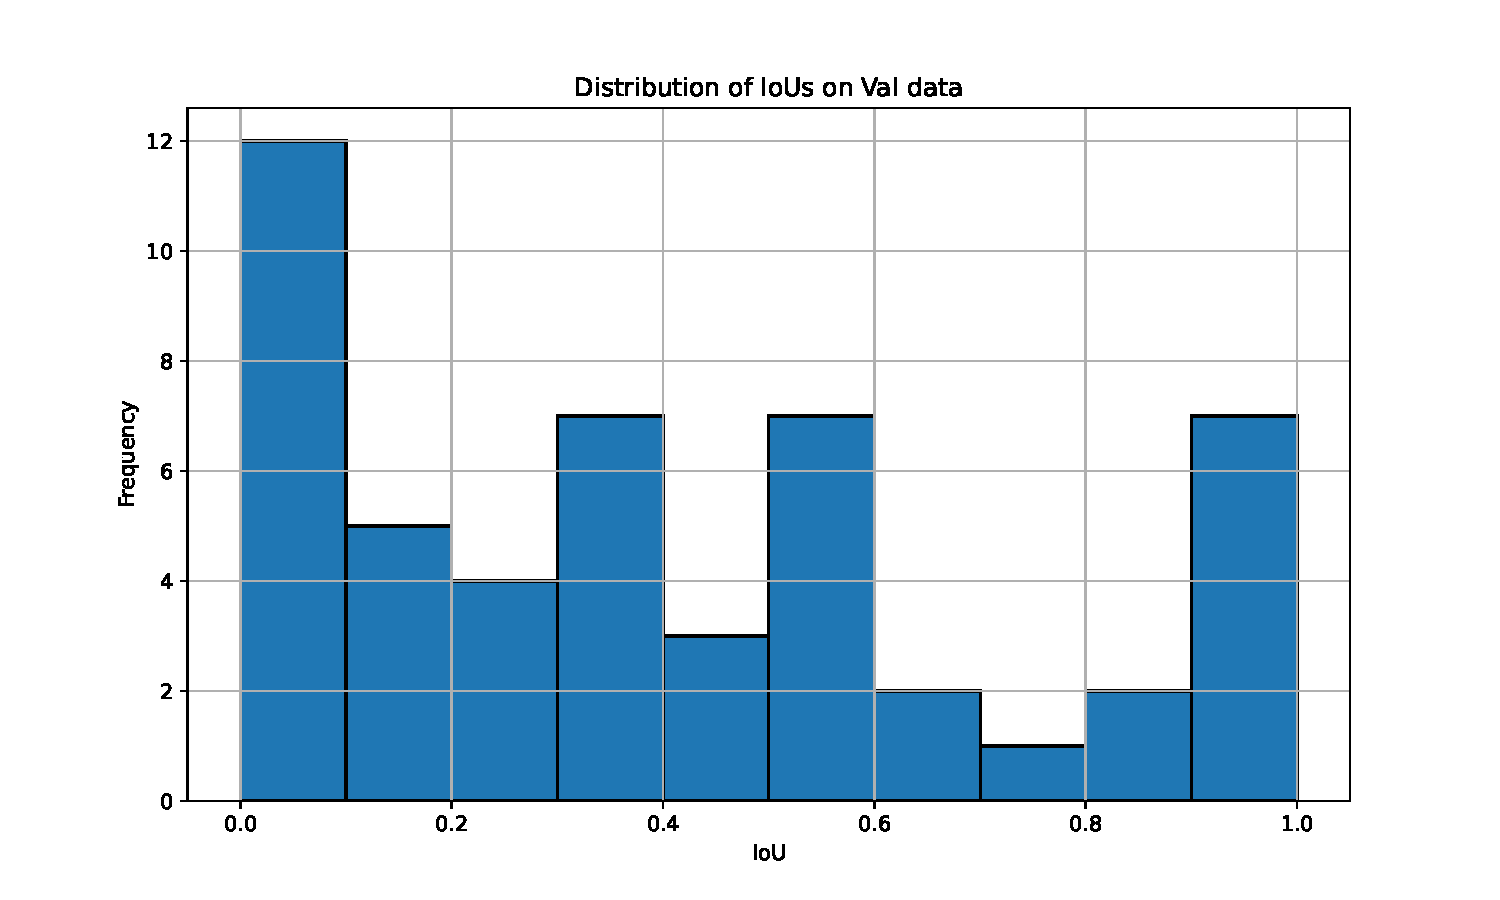
\includegraphics[width=\textwidth]{images/ious_histogram.pdf}
    \caption{распределение IoU на объектах SemEval-2025.}
    \label{fig:ious_histogram}
\end{figure}

\clearpage
\section{Заключение}

В данной работе были рассмотрены разные векторные представления фрагментов для задачи классификации связей, а также рассмотрен подход MRC. В результате экспериментов самым лучшим по $F_1$ с микро усреднением оказался метод MRC с векторным представлением фрагментов, которое строится усреднением через механизм внимания.

Был предложен критерий оценки качества моделей для совместного выделения сущностей и фрагментов, который сглаживает F-меру и позволяет лучше оценить качество разметки. Лучший результат показал подход MRC.
Основная проблемма методов - низкое качество поиска релевантных пар фрагментов.

Дальнейшая работа связана с улучшением качества совместного выделения фрагментов и связей между ними. \cite{abaho2021detect}
\clearpage

\bibliographystyle{splncs04}
\bibliography{references}

\clearpage
\section{Приложение}

\end{document}